\section*{Введение}
\addcontentsline{toc}{section}{Введение}
В последнее время всё более широкое распространение в различных областях науки и техники получает применение композиционных материалов. 
Из них изготавливается спортивное и медицинское оборудование, детали двигателей, обшивка и силовые конструкции корпусов самолётов и космических аппаратов, 
бронежилеты и элементы брони военной техники, детали и кузова автомобилей.

Композиционный материал - неоднородный сплошной материал, состоящий из двух или более компонентов с чёткой границей раздела между ними.
Правильное комбинирование нескольких элементов, каждый из которых обладает неким выдающимся качеством, позволяет получить материал, 
совмещающий эти свойства или близкий к этому, а также, возможно, имеющий новые интересные свойства \cite{resler}.

Интенсивное использование материалов приводит к их износу и выходу из строя выполненных из них конструкций. Как правило, серьёзные разрушения происходят не
внезапно, им предшествует накопление и рост дефектов внутри материала. Однако очень часто обнаружить такие дефекты невозможно без применения специальных
средств. 

Неразрушающий контроль - проверка надежности основных рабочих параметров объекта или отдельных его элементов, не требующая выведения объекта из работы либо его демонтажа.
Существует множество методов, среди которых акустические, тепловые, радиационные, радиоволновые, проникающими веществами и другие.

Акустический, он же, в зависимости от частоты, ультразвуковой способ основан на регистрации и анализе параметров упругих волн в объекте контроля. Выделяют пассивный, при котором анализируются существующие в образце шумы, и активный, основанный на измерении интенсивности пропускаемого или отражаемого сигнала.

Большинство существующих методов анализа показаний прибора акустического неразрушающего контроля - ультразвукового дефектоскопа - основывается на так называемом лучевом приближении, аналогичном геометрической оптике. Во многих случаях это даёт необходимый результат. Однако в сложных случаях, связанных с анизотропными и композиционными  материалами и  множественными дефектами, результат не всегда удовлетворителен.

В связи с этим предлагается провести более глубокий анализ волновых процессов, происходящих при акустическом неразрушающем контроле, проведя прямое численное моделирование этого процесса в рамках модели механики дефрмируемого твёрдого тела. Сеточно\hyp{}характеристический численный метод, напрямую учитывающий волновые свойства уравнений математической модели, подходит для этого как нельзя лучше.

При распространении акустических волн в среде деформации пренебрежимо малы. Из этого следует два факта. Во-первых, для математического описания задачи подходит линейная теория упругости. Во-вторых, расчётная сетка численного метода может быть выбрана неподвижной. Это, однако, не даёт возможности полностью ограничиться структурированными сетками, так как они не позвлоляют смоделировать дефекты произвольной формы.

Таким образом, данная работа посвящена применению сеточно\hyp{}характеристического метода к расчёту распространения акустических волн в линейно-упругом теле. Рассматриваются задачи с анизотропией упругих свойств материала, наличием внутренних дефектов, слоистыми материалами. 

Проведены расчёты постановок с параметрами, близкими к параметрам реальных производственных ситуаций неразрушающего контроля композитных материалов (расчёт обшивки представленного на рис. \ref{pic:construction} элемента крыла самолёта).

\begin{figure}[H]
	\center{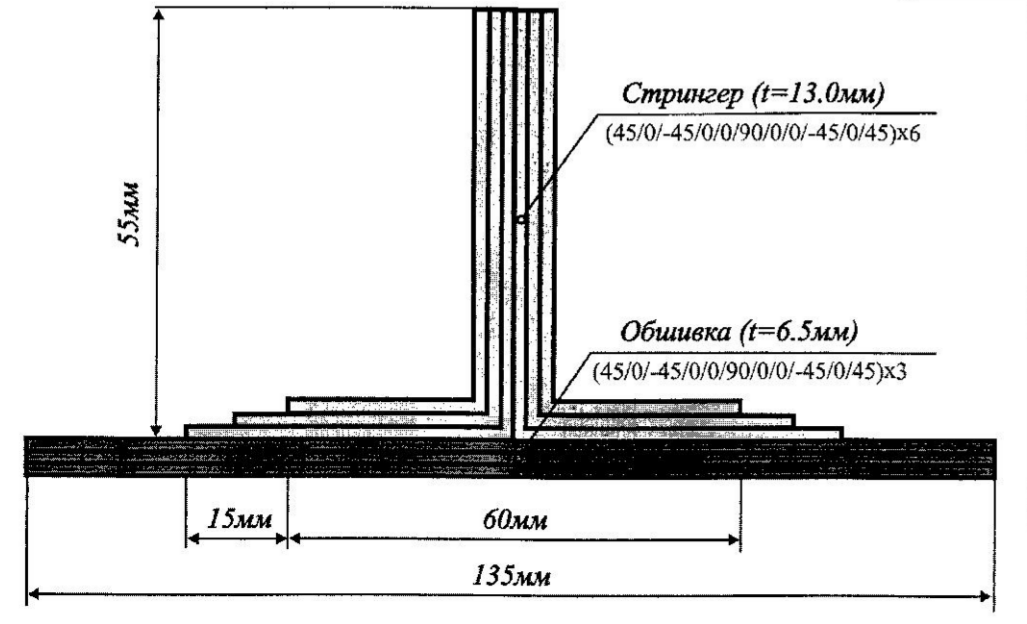
\includegraphics[width=1\textwidth]{png/construction.png}}
	\caption{Образец}
	\label{pic:construction}
\end{figure}